% !TEX TS-program = XeLaTeX
% use the following command:
% all document files must be coded in UTF-8
\documentclass[spanish]{textolivre}
% build HTML with: make4ht -e build.lua -c textolivre.cfg -x -u article "fn-in,svg,pic-align"

\journalname{Texto Livre}
\thevolume{18}
%\thenumber{1} % old template
\theyear{2025}
\receiveddate{\DTMdisplaydate{2024}{12}{20}{-1}} % YYYY MM DD
\accepteddate{\DTMdisplaydate{2025}{4}{29}{-1}}
\publisheddate{\DTMdisplaydate{2025}{6}{10}{-1}}
\corrauthor{Mario Cerezo-Pizarro}
\articledoi{10.1590/1983-3652.2025.56657}
%\articleid{NNNN} % if the article ID is not the last 5 numbers of its DOI, provide it using \articleid{} commmand 
% list of available sesscions in the journal: articles, dossier, reports, essays, reviews, interviews, editorial
\articlesessionname{articles}
\runningauthor{Cerezo-Pizarro, Revuelta-Domínguez y Guerra-Antequera} 
%\editorname{Leonardo Araújo} % old template
\sectioneditorname{Hugo Heredia Ponce}
\layouteditorname{Daniervelin Pereira}

\title{Videojuegos en las aulas: un estudio evaluativo sobre un curso de formación en la utilización de videojuegos para el profesorado extremeño}
\othertitle{Videogames na sala de aula: um estudo avaliativo de um curso de treinamento sobre o uso de videogames para professores na Extremadura}
\othertitle{Video games in the classroom: an evaluative study of a training course on the use of video games for teachers in Extremadura}
% if there is a third language title, add here:
%\othertitle{Artikelvorlage zur Einreichung beim Texto Livre Journal}

\author[1]{Mario Cerezo-Pizarro~\orcid{0000-0001-8097-0573}\thanks{Email: \href{mailto:mariocp@unex.es}{mariocp@unex.es}}}
\author[1]{Francisco Ignacio Revuelta-Domínguez~\orcid{0000-0002-3649-4327}\thanks{Email: \href{mailto:fird@unex.es}{fird@unex.es}}}
\author[1]{Jorge Guerra-Antequera~\orcid{0000-0003-1675-8038}\thanks{Email: \href{mailto:guerra@unex.es}{guerra@unex.es}}}
\affil[1]{Universidad de Extremadura, Extremadura, España.}

\addbibresource{article.bib}
% use biber instead of bibtex
% $ biber article

% used to create dummy text for the template file
\definecolor{dark-gray}{gray}{0.35} % color used to display dummy texts
\usepackage{lipsum}
\SetLipsumParListSurrounders{\colorlet{oldcolor}{.}\color{dark-gray}}{\color{oldcolor}}

% used here only to provide the XeLaTeX and BibTeX logos
\usepackage{hologo}

% if you use multirows in a table, include the multirow package
\usepackage{multirow}

% provides sidewaysfigure environment
\usepackage{rotating}

% CUSTOM EPIGRAPH - BEGIN 
%%% https://tex.stackexchange.com/questions/193178/specific-epigraph-style
\usepackage{epigraph}
\renewcommand\textflush{flushright}
\makeatletter
\newlength\epitextskip
\pretocmd{\@epitext}{\em}{}{}
\apptocmd{\@epitext}{\em}{}{}
\patchcmd{\epigraph}{\@epitext{#1}\\}{\@epitext{#1}\\[\epitextskip]}{}{}
\makeatother
\setlength\epigraphrule{0pt}
\setlength\epitextskip{0.5ex}
\setlength\epigraphwidth{.7\textwidth}
% CUSTOM EPIGRAPH - END

% to use IPA symbols in unicode add
%\usepackage{fontspec}
%\newfontfamily\ipafont{CMU Serif}
%\newcommand{\ipa}[1]{{\ipafont #1}}
% and in the text you may use the \ipa{...} command passing the symbols in unicode

% LANGUAGE - BEGIN
% ARABIC
% for languages that use special fonts, you must provide the typeface that will be used
% \setotherlanguage{arabic}
% \newfontfamily\arabicfont[Script=Arabic]{Amiri}
% \newfontfamily\arabicfontsf[Script=Arabic]{Amiri}
% \newfontfamily\arabicfonttt[Script=Arabic]{Amiri}
%
% in the article, to add arabic text use: \textlang{arabic}{ ... }
%
% RUSSIAN
% for russian text we also need to define fonts with support for Cyrillic script
% \usepackage{fontspec}
% \setotherlanguage{russian}
% \newfontfamily\cyrillicfont{Times New Roman}
% \newfontfamily\cyrillicfontsf{Times New Roman}[Script=Cyrillic]
% \newfontfamily\cyrillicfonttt{Times New Roman}[Script=Cyrillic]
%
% in the text use \begin{russian} ... \end{russian}
% LANGUAGE - END

% EMOJIS - BEGIN
% to use emoticons in your manuscript
% https://stackoverflow.com/questions/190145/how-to-insert-emoticons-in-latex/57076064
% using font Symbola, which has full support
% the font may be downloaded at:
% https://dn-works.com/ufas/
% add to preamble:
% \newfontfamily\Symbola{Symbola}
% in the text use:
% {\Symbola }
% EMOJIS - END

% LABEL REFERENCE TO DESCRIPTIVE LIST - BEGIN
% reference itens in a descriptive list using their labels instead of numbers
% insert the code below in the preambule:
%\makeatletter
%\let\orgdescriptionlabel\descriptionlabel
%\renewcommand*{\descriptionlabel}[1]{%
%  \let\orglabel\label
%  \let\label\@gobble
%  \phantomsection
%  \edef\@currentlabel{#1\unskip}%
%  \let\label\orglabel
%  \orgdescriptionlabel{#1}%
%}
%\makeatother
%
% in your document, use as illustraded here:
%\begin{description}
%  \item[first\label{itm1}] this is only an example;
%  % ...  add more items
%\end{description}
% LABEL REFERENCE TO DESCRIPTIVE LIST - END


% add line numbers for submission
%\usepackage{lineno}
%\linenumbers

\begin{document}
\maketitle

\begin{polyabstract}
\begin{abstract}
La introducción de los videojuegos en las aulas es un reto pendiente en la formación del profesorado. Esta necesidad, detectada y fundamentada tanto por los investigadores como por los responsables educativos, avala el planteamiento y desarrollo de cursos especializados. El presente estudio enuncia la labor realizada en colaboración con los Centros de Profesores y Recursos de la comunidad autónoma de Extremadura, España, mediante el desarrollo y análisis del proceso de implantación y desarrollo 4 cursos de formación. A través de un diseño de investigación evaluativa de carácter mixto, se somete a evaluación este proceso, considerando el desarrollo de estas formaciones como una herramienta fundamental de cara a la adaptación curricular y la integración del videojuego en las aulas. Para alcanzar conclusiones al respecto, se examinan las percepciones y experiencias de 59 docentes. Los resultados permiten identificar los perfiles más interesados en este tipo de formación, así como las expectativas y el grado de satisfacción respecto a la adecuación, adaptación y aplicación práctica del videojuego en el contexto educativo extremeño. De esta manera, se somete a evaluación la propia formación, permitiendo identificar y exponer un modelo formativo adaptado a las necesidades y demandas del profesorado. El proceso de evaluación permite destacar la mayor idoneidad de formaciones presenciales frente a otros modelos de enseñanza, así como el interés del profesorado por crear sus propios videojuegos y experiencias docentes que se contrasta en gran medida con la ausencia de formación específica y las dificultades encontradas a la hora de seleccionar recursos de terceros.

\keywords{Videojuego \sep Docente \sep Formación \sep Curso de enseñanza \sep Asociación de profesores}
\end{abstract}

\begin{portuguese}
\begin{abstract}
A introdução de videogames na sala de aula é um desafio pendente na formação de professores. Essa necessidade, detectada e apoiada tanto por pesquisadores quanto por líderes educacionais, apoia o planejamento e o desenvolvimento de cursos especializados. Este estudo apresenta o trabalho realizado em colaboração com os Centros de Professores e Recursos da comunidade autônoma de Extremadura, Espanha, por meio do desenvolvimento e da análise do processo de implementação e desenvolvimento de 4 cursos de treinamento. Por meio de um projeto de pesquisa avaliativa mista, esse processo é avaliado, considerando o desenvolvimento desses cursos de treinamento como uma ferramenta fundamental para a adaptação curricular e a integração de videogames na sala de aula. Para chegar a conclusões a esse respeito, são examinadas as percepções e experiências de 59 professores. Os resultados nos permitem identificar os perfis mais interessados nesse tipo de treinamento, bem como as expectativas e o grau de satisfação em relação à adequação, adaptação e aplicação prática do videogame no contexto educacional da Extremadura. Dessa forma, o próprio treinamento é submetido à avaliação, o que permite identificar e expor um modelo de treinamento adaptado às necessidades e demandas do corpo docente. O processo de avaliação destaca a maior adequação do treinamento presencial em comparação com outros modelos de ensino, bem como o interesse dos professores em criar seus próprios videogames e experiências de ensino, o que contrasta em grande parte com a ausência de treinamento específico e as dificuldades encontradas ao selecionar recursos de terceiros.

\keywords{Videogame \sep Professor \sep Treinamento \sep Curso de ensino \sep Associação de professores}
\end{abstract}
\end{portuguese}

\begin{english}
\begin{abstract}
The introduction of video games in the classroom is a pending challenge in teacher training. This need, detected and supported by both researchers and educational leaders, supports the planning and development of specialised courses. This study sets out the work carried out in collaboration with the Teachers and Resources Centres of the autonomous community of Extremadura, Spain, through the development and analysis of the process of implementation and development of 4 training courses. Through a mixed evaluative research design, this process is evaluated, considering the development of these training courses as a fundamental tool for curricular adaptation and the integration of video games in the classroom. In order to reach conclusions in this respect, the perceptions and experiences of 59 teachers are examined. The results allow us to identify the profiles most interested in this type of training, as well as the expectations and degree of satisfaction with regard to the suitability, adaptation and practical application of the video game in the educational context of Extremadura. In this way, the training itself is subjected to evaluation, making it possible to identify and expose a training model adapted to the needs and demands of the teaching staff. The evaluation process makes it possible to highlight the greater suitability of face-to-face training compared to other teaching models, as well as the interest of teachers in creating their own video games and teaching experiences, which contrasts to a large extent with the absence of specific training and the difficulties encountered when selecting third-party resources.

\keywords{Video games \sep Teacher \sep Training \sep Teaching course \sep Teachers' association}
\end{abstract}
\end{english}
% if there is another abstract, insert it here using the same scheme
\end{polyabstract}

\section{Introducción}\label{sec-intro}
La implementación del videojuego en las aulas nunca ha estado exenta de dificultades. El primer escollo a superar fue la visión social del videojuego como medio educativo, vinculada a las raíces y percepciones negativas que durante décadas han existido frente a su uso en las aulas \cite{moreno2025violence,nunez2020videojuegos}. Aunque algunos autores encuentran todavía efectos negativos en la interrelación entre videojuegos, educación y resultados académicos \cite{carrillo2022consumo}, son más numerosas las investigaciones que, frente a ello, destacan los aspectos positivos de una utilización estructurada y organizada del medio como recurso educativo \cite{cole2024scoping,granic2014benefits,martinez2022entertainment,mielgo2022revision,rodriguez2002jovenes}, destacando aspectos como el aumento de la motivación \cite{gordillo2022comparing,tacoronte2023systematic}, la adquisición de habilidades y competencias específicas, la posibilidad de realizar simulaciones y situaciones de aprendizaje dentro de contextos seguros \cite{arias2014using,buil2019encouraging,kashiwakura2008jogando} o trabajar por la educación inclusiva y la mejora del acceso al aprendizaje \cite{screpnik2024educacion}.

En cuanto a su implementación en las aulas, existe una amplia revisión de la literatura \cite{boyle2016update,connolly2012systematic,grande2018beneficios,guerra2022investigacion} que enuncia las posibilidades, áreas y recursos utilizados para conseguir una interrelación positiva entre videojuegos y aprendizaje, permitiendo a los docentes replicar  intervenciones y propuestas educativas e identificar los elementos, dificultades y metodologías más importantes \cite{marklund2016educational,tsekleves2016benefits}.

En todos estos estudios, además del esfuerzo adicional para el profesorado y las dificultades para argumentar el uso de videojuegos ante padres y administración educativa, siempre se destaca la necesidad de recursos y la vinculación entre la formación específica \cite{gonzalez2023diseno} y la posterior implementación del videojuego en las aulas \cite{correa2016horizontes,cozar2024ensenar,lorca2016utilidad,marin2022videojuegos}.

Es necesario señalar que, aunque existe una amplia oferta de videojuegos y recursos en el mercado, no todos pueden catalogarse como videojuegos educativos, al no contar en su desarrollo con una clara intencionalidad educativa, ni estar adaptados a la etapa o contenidos que se desean trabajar \cite{estallo1995videojuegos}. Esto implica un reto enorme para el profesorado, pues debe no solo ser capaz de seleccionar, testear e introducir videojuegos en el aula, sino que además, debe conseguir que estos sean motivadores y desarrollen aprendizajes significativos en su alumnado. En este sentido, la investigación académica ha comenzado a ofrecer recursos al profesorado, como la guía creada por \textcite{lopez2023videojuegos} en la que se exponen algunas de las claves para integrar el videojuego en el aula, destacando también la idoneidad de que el profesorado sea capaz de crear sus propios videojuegos.

De hecho, una investigación realizada durante el curso 2018/2019 por \textcite{gonzalez2023diseno} analizó el diseño y programación de un videojuego educativo en Educación Primaria, descubriendo que implicar al alumnado en el uso de videojuegos en las aulas ofrecía beneficios personales, curriculares y profesionales. Mientras que \textcite{gerardo2022videojuego} enuncian el interés del profesorado más joven en la aplicación didáctica del videojuego y las limitaciones formativas encontradas por el resto de los docentes para su implementación.

Teniendo en cuenta tanto los elementos positivos que emergen del uso educativo del videojuego como la necesidad de formación al respecto, resulta procedente desarrollar una oferta educativa específica destinada al profesorado que quiera aprender a programar y diseñar sus propios videojuegos y trasladar sus conocimientos al aula \cite{gonzalez2023diseno}.

\section{Videojuegos en las aulas extremeñas}\label{sec-normas}
El uso de videojuegos en las aulas es una tendencia educativa que como consecuencia de la popularidad del medio y las posibilidades didácticas que ofrece se está extendiendo por todo el mundo \cite{mielgo2022revision}. En el contexto autonómico, existen ya investigaciones como la de \textcite{pedrera2017percepcion} que recogió por primera vez datos sobre las percepciones del alumnado del Grado en Educación Infantil de la Universidad de Extremadura en torno al uso de videojuegos en línea y sus implicaciones en el desarrollo de habilidades y competencias, encontrando implicaciones en aspectos como la toma de decisiones, la competencia interpersonal, la psicomotricidad o la atención.

En el año 2018, un estudio desarrollado en la Universidad de Extremadura evaluó las percepciones y opiniones del alumnado de 4º de la ESO en torno al contenido histórico de un videojuego de realidad virtual, así como el valor pedagógico que le atribuían, encontrando una recepción positiva por parte de los participantes hacia los contenidos, así como el valor añadido de su utilización como elemento de motivación \cite{martinezsoto2018evaluacion}, mientras que otro estudio encontró relaciones positivas entre el uso de videojuegos y los niveles de fluidez y capacidad lectora en niños de entre 6 y 8 años con dificultades de aprendizaje o dislexia \cite{jimenez2018impacto}.

Más recientemente, investigadores de la Universidad de Extremadura han expuesto la relación positiva entre el uso de los videojuegos y el desarrollo de habilidades blandas en 247 estudiantes universitarios, demostrando la capacidad de los videojuegos de impactar en el rendimiento académico \cite{alloza2022genre}, mientras que un proyecto de la Fundación COTEC para la innovación, financió el desarrollo de un videojuego para combatir las noticias falsas y la desinformación \cite{cotec2022anuario}.

De este modo, el interés del profesorado en la aplicación didáctica del videojuego, así como la integración o validación de este recurso que se está realizando desde las universidades y organismos de investigación e innovación fomenta el desarrollo de formaciones específicas para el profesorado en activo, que respondan a las demandas de docentes, sociedad e investigación educativa.

\subsection{Formación del profesorado en Extremadura. La detención de necesidades formativas en los Centros de Profesores y Recursos}

La gestión y organización de las actividades de formación del profesorado en la comunidad autónoma de Extremadura depende de los Centros de Profesores y Recursos, en adelante CPR, centros dependientes de la Consejería de Educación y Empleo, que a su vez pertenecen a la Dirección General de Innovación e Inclusión Educativa.

Su labor es elaborar y desarrollar planes de formación para el profesorado dependiente de la administración autonómica, mejorando y potenciando las prácticas, metodologías y funciones docentes. Para ello, la comunidad autónoma de Extremadura cuenta con un total de 18 CPR, distribuidos por las distintas áreas geográficas, que permiten una programación de actividades acorde a las necesidades de desplazamiento del profesorado. No obstante, la participación en los cursos no se limita directamente al ámbito o demarcación geográfica de cada CPR, sino que estos están abiertos a toda la comunidad.

Anualmente, en base a las demandas del profesorado, los CPR desarrollan un Plan de Formación que incluye: cursos, cursos a distancia, grupos de trabajo, seminarios, jornadas y congresos. La elección y el desarrollo de las actividades dentro de los Centros de Profesores y Recursos es un proceso estructurado que se basa en 4 pilares que, en este caso, sirven para justificar tanto el desarrollo del curso como la investigación posterior: el primero de ellos (1) es la detección de necesidades formativas que se realiza a través de formularios que cada CPR brinda a los distintos centros educativos de su demarcación geográfica con el objetivo de recoger el sentir de los claustros. Seguidamente, estas propuestas se recogen y estructuran en torno a la normativa de aplicación (2) a través del Plan Marco Regional de Formación Permanente del Profesorado, donde se establecen las líneas directrices que desde la Consejería de Educación y Empleo se estructuran \cite{extremadura2016plan} sirviendo para elaborar el Plan Regional de Formación Permanente del Profesorado \cite{extremadura2022plan}, donde se recogen las líneas prioritarias de formación. La comunidad autónoma de Extremadura recoge la investigación e innovación educativa para el desarrollo de nuevas metodologías de enseñanza, fomentando el propio centro educativo como marco y la aplicación al aula como referente, así como la sostenibilidad y la transferencia de las mejoras, o la consolidación y ampliación en el manejo y uso de aplicaciones didácticas. De esta manera, se da continuidad a la necesidad detectada en primera instancia de entender y utilizar los videojuegos en el aula, algo que (3) los responsables de formación de cada centro verifican a través de las líneas de actuación y el interés del profesorado. Siendo clave en última instancia (4) el interés real del profesorado y el número de solicitudes o matrículas que cada curso recibe una vez publicado.


\subsection{Aplicación de los videojuegos en el ámbito educativo}\label{sec-fmt-manuscrito}
Para realizar esta investigación fue necesario diseñar y plantear un curso práctico enfocado a la integración de los videojuegos como recurso de aula. En este sentido se planteó durante el año 2021 una primera edición desarrollada en el CPR de Zafra del curso titulado: \textit{Aplicación de los videojuegos en el ámbito educativo}, que constaba de 12 horas teórico-prácticas en las que se presentaban las ventajas e inconvenientes del uso de videojuegos en el aula, la aproximación al concepto, la exposición de experiencias y posibilidades de prácticas, así como la introducción del profesorado en el diseño y utilización de videojuegos específicos que permitieran incorporar este recurso en sus aulas.

En base al éxito y la aceptación de esta primera edición entre el profesorado extremeño y bajo petición expresa de los Centros de Profesores y Recursos, se han desarrollado desde entonces un total de 4 ediciones distribuidas en 3 CPR distintos (Zafra, Badajoz y Trujillo). Las distintas ediciones siempre han mantenido su duración, variando únicamente el factor de presencialidad, desde una primera edición con componente online condicionada por la COVID-19, que pasó a semipresencial, para finalmente convertirse en un curso presencial. La información de dichos cursos se ha publicado en las páginas web y los planes de formación de los distintos centros \cite{cprzafra2021videojuegos} y la aceptación de los cursos se ha reflejado en la repetición y transferencia existente entre los distintos CPR, dada la innovación y la actualidad de la propuesta que llegó a aparecer en la prensa local \cite{diariohoy2022curso}.


\subsection{Propósito del estudio, objetivos y preguntas de investigación}\label{sec-formato}
La investigación en educación debe acompañarse de propuestas y actividades específicas \cite{counsell2000usefulness,gonzalez2023diseno}. En este sentido, el planteamiento de estos cursos de formación responde a las necesidades y demandas del profesorado a la vez que permite desarrollar un área de investigación en curso, dentro de la Tesis Doctoral de Mario Cerezo Pizarro. Partiendo de esta premisa, se constituye un grupo de trabajo que permite el planteamiento y desarrollo de las diferentes ediciones de este curso. Tras cada edición, y en colaboración con los CPR, se elabora y realiza una encuesta de valoración de la actividad que permite tanto al Centro de Profesores y Recursos como a los investigadores, evaluar la actividad, su implementación y grado de éxito, así como desarrollar una investigación estructurada en torno al interés, las posibles mejoras y la adecuación de estas formaciones en la comunidad autónoma de Extremadura. Los objetivos de esta investigación son los siguientes:

\begin{itemize}
    \item Realizar un análisis de la situación del profesorado extremeño en relación con la predisposición de aprender o utilizar videojuegos en el aula.
    \item Desarrollar y evaluar un modelo de formación para el profesorado de cara a la implementación escolar del videojuego.
    \item Identificar elementos claves a la hora de utilizar videojuegos en las aulas, formando al profesorado y teniendo en cuenta sus necesidades y opiniones.
\end{itemize}

En base a ellos se plantean una serie de preguntas (en adelante P) e intereses específicos de investigación, enumeradas a continuación:

\begin{enumerate}
    \item[P1.] ¿Qué profesorado muestra interés por las formaciones específicas vinculadas a la utilización de los videojuegos en el aula?, ¿cuáles son sus perfiles académico-profesionales?
    \item[P2.] ¿Qué expectativas tiene el profesorado extremeño en relación con la incorporación de los videojuegos a su formación y práctica educativa?
    \item[P3.] ¿Qué grado de satisfacción muestran respecto al curso de \textit{Aplicación de los videojuegos en el ámbito educativo}?
    \item[P4.] ¿Se adecua este tipo de formación a sus puestos de trabajo y a la formación profesional que los docentes perciben como necesaria?
    \item[P5.] ¿Qué valoración media recibe la actividad de formación?
    \item[P6.] ¿Qué percepciones individuales tiene el profesorado extremeño sobre el desarrollo de este curso?, ¿qué propuestas de mejora o evaluaciones cualitativas realizan?
    \item[P7.] ¿Qué aspectos o elementos del curso fueron necesarios mejorar o cambiar?, ¿qué elementos identifica como determinantes en el proceso de aprendizaje-utilización el profesorado participante?
\end{enumerate}

\section{Método}\label{sec-modelo}
Esta investigación presenta un estudio evaluativo de carácter mixto en el que se recogen datos de carácter cuantitativo y cualitativo en torno al diseño y desarrollo de una serie de cursos sobre la aplicación didáctica de los videojuegos en el aula realizados en los Centros de Profesores y Recursos de las localidades de Zafra, Badajoz y Trujillo.

La elección de la investigación evaluativa se fundamenta en las características y ventajas que esta metodología ofrece a la hora de analizar las necesidades educativo-formativas de un grupo específico \cite{bausela2004metodologia}. En este caso se analiza al profesorado extremeño a través de su propia formación, considerando que la posibilidad de trasladar los aprendizajes adquiridos al aula se vincula directamente con el desarrollo de las competencias necesarias para hacerlo. Se pretende así establecer relaciones entre los docentes extremeños y la implementación de los videojuegos en sus aulas, buscando definir un modelo para mejorar esta implementación. La investigación evaluativa permite hacerlo, estructurando un proceso de análisis y evaluación del mismo para tomar decisiones de desarrollo y mejora, así como para establecer criterios que determinen la adecuación o no de los programas y diseños de investigación \cite{escudero2016investigacion}.

\subsection{Participantes}\label{sec-organizacao}
En este estudio participaron 59 docentes, pertenecientes a cada una de las cuatro ediciones en las que se desarrolló el curso. Cabe recordar que solo se analizan los datos de aquellas personas que además de inscribirse y completar el curso, deciden voluntariamente hacerlo, por lo que se está utilizando un muestreo no probabilístico denominado como muestreo incidental. Este muestreo se caracteriza por realizarse en situaciones en las que no se controla directamente la muestra, utilizándose habitualmente para estudiar fenómenos raros o inusitados que se analizan con relación a la presencialidad o vinculación casuística no procedimental del estudio \cite{hernandez2019muestreo}. La correlación del número de participantes, su género, edad, experiencia docente y tipología de centro al que pertenecen se expone en la siguiente tabla (Ver \Cref{tbl1}).

\begin{table}[htbp]
\centering
\begin{threeparttable}
\caption{Datos sociodemográficos de la muestra.}
\label{tbl1}
\begin{tabular}{llll}
\toprule
Variable & Categoría & Frecuencia & Porcentaje  \\ 
 \midrule
\multirow{2}{*}{Género} & Masculino & 23 & 39.98~\%  \\ 
& Femenino & 36 & 61.02~\%   \\ 
\multirow{3}{*}{Edad} & Menos de 25 años & 2 & 3.39~\% \\
& Entre 25 y 45 años & 42 & 71.19~\% \\
& Mayores de 45 años & 15 & 25.42~\% \\
\multirow{5}{*}{Experiencia docente} & De 1 a 5 años & 34 & 57.63~\% \\
& De 6 a 10 años & 4 & 6.78~\% \\
& De 11 a 15 años & 8 & 13.56~\% \\
& De 16 a 20 años & 5 & 8.47~\% \\
& Más de 20 años & 8 & 13.56~\% \\
\multirow{2}{*}{Titularidad del centro} & Público & 55 & 93.22~\% \\
& Privado & 4 & 6.78~\% \\
\multirow{2}{*}{Relación contractual} & Interinos & 33 & 55.93~\% \\
& Otras situaciones & 26 & 44.07~\% \\
\multirow{3}{*}{Etapa o cuerpo docente} & Maestros & 19 & 32.20~\% \\
& Secundaria & 35 & 59.32~\% \\
& Formación Profesional & 5 & 8.47~\% \\
\bottomrule
\end{tabular}
\source{Elaboración propia.}
\end{threeparttable}
\end{table}



\subsection{Procedimiento}\label{sec-organizacao-latex}
De forma concreta, los pasos a seguir en cada una de las fases fueron los siguientes:
\begin{enumerate}
    \item[Fase 1)] detección de necesidades formativas y planteamiento del curso: se inicia el contacto con los CPR, detectando las necesidades formativas del profesorado y planteándoles la posibilidad de desarrollar una formación específica en torno a la aplicación didáctica de los videojuegos en el aula. Esta fase implica la creación y publicación de una propuesta de actividad formativa que debe superar dos filtros: primeramente, debe ser aceptada por los responsables de las áreas formativas y la dirección del CPR, para después ser publicitada y anunciada dentro de sus planes de formación; en ese caso, y solo si la demanda de participantes es suficiente, el curso se lleva a cabo.
    \item[Fase 2)] desarrollo y conceptualización del curso: Se inicia con la creación de la ficha inicial y se culmina con la aceptación del curso, en este momento es necesario configurar un equipo de ponentes, delimitar los aspectos y metodologías a trabajar y estructurar la carga horaria del curso. La información de las fichas se expone para su consulta y difusión en las webs de los CPR, sirva de ejemplo la del último curso realizado: \url{https://bit.ly/3XVX9wa}, \url{https://rfp.educarex.es/pub/archivos/dipticos/21/2022/79292-diptico.pdf}.
    \item[Fase 3)] Desarrollo de la actividad formativa: Incluye la realización de la propia actividad (Ver \Cref{fig1}), su promoción \url{https://twitter.com/cpr_zafra/status/1456587188217470976?s=21} y difusión: \url{https://twitter.com/cpr_zafra/status/1456517315328086018?s=21}.

    \begin{figure}
    \centering
    \begin{minipage}{0.75\linewidth}
    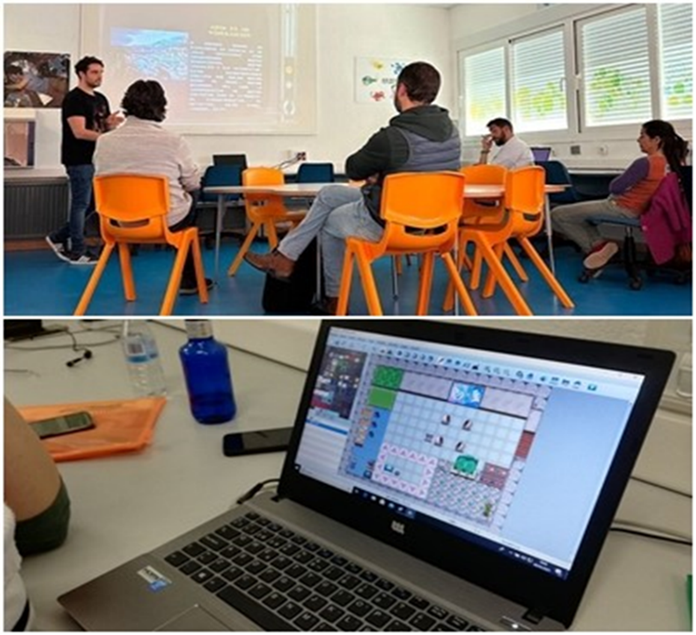
\includegraphics[width=\linewidth]{Fig1.png}
    \caption{Sesiones de Formación en videojuegos y su aplicación didáctica. CPR de Zafra.}
    \label{fig1}
    \source{Imagen propia.}
    \end{minipage}
    \end{figure}

    \item[Fase 4)] recepción de información evaluativa y reestructuración de los contenidos y metodologías aplicadas: el custodio y la recogida de información fue realizada por los CPR que ceden los datos anonimizados para analizarlos y agruparlos en esta investigación. De este modo, si el curso se reedita, es posible mejorar y analizar.

    \item[Fase 5)] exposición de resultados y conclusiones: Los datos recabados durante todo el proceso de investigación se analizan y reinterpretan para obtener macro-conclusiones.
\end{enumerate}
 

 

 



 



\subsection{Técnicas e instrumentos de análisis de datos}\label{sec-titulo}
La recogida de información se realiza desde los propios Centros de Profesores y Recursos con quien se establece el acuerdo personal de transferencia de datos. Posteriormente, la institución cede estos a los investigadores, acordando, que serán utilizados en una investigación más amplia. Se trata de datos anonimizados que garantizan la seguridad de estos, condicionados al procedimiento de recogida utilizado dentro de estos centros, lo que en muchos casos implica trabajar con las medias. Así, el cuestionario utilizado se compone de 4 secciones, la primera de ellas destinada a recoger datos estadísticos sobre los participantes, recoge: edad, experiencia docente, sexo, titularidad del centro y otros datos sobre la situación administrativa y la etapa en la que imparten enseñanza los participantes. La segunda se centra en las expectativas respecto a la formación del profesorado, indagando en cuestiones como la necesidad de formación, su utilidad como mérito y complemento docente frente a la mejora de la competencia profesional y la propia práctica educativa. Seguidamente, la herramienta evalúa la propia actividad: duración, horario, organización, uso de materiales y equipamientos, metodología, etcétera. Finalmente, permite un espacio de carácter cualitativo a través de un apartado de propuestas de mejora, en las que el profesorado puede transmitir sus percepciones y valoraciones de forma anónima. El modelo del cuestionario es el siguiente: \url{https://figshare.com/articles/dataset/Modelo_de_evaluaci_n_CPR/25112027}.

\section{Resultados}\label{sec-autores}
Para enunciar los resultados de esta investigación se toman como referencia las preguntas de estudio planteadas inicialmente, estructurando en torno a ellas la exposición de los resultados. Conviene añadir que el carácter evaluativo de la investigación y del curso de formación implica el rediseño total o parcial de algunos aspectos de la formación, lo que se reseña debidamente en la P7. Los datos se encuentran disponibles en: \url{https://figshare.com/articles/dataset/Analisis_de_datos_Media_cursos_videojuegos_CPR_-_Extremadura/25112036}.

\subsection{P1. ¿Qué profesorado muestra interés por las formaciones vinculadas a la utilización de los videojuegos?}\label{sec-idioma}
La inscripción y participación en los cursos de formación ofertados por los CPR de Extremadura permite definir los perfiles del profesorado de la comunidad autónoma en relación con el interés y la predisposición que estos muestran por incluir videojuegos en sus aulas. El análisis realizado en esta investigación muestra que la edad media del profesorado interesado en los videojuegos oscila entre 25 y 45 años; lo que supone un total de 42 participantes, el 71.2~\%, estaban en este rango de edad, frente a solo 15 de los 59 (25.4~\%) de participantes que superaban los 45 años y 2 que eran menores de 25 años (3.4~\%) (\Cref{fig2}).

\begin{figure}[h!]
    \centering
    \begin{minipage}{0.75\linewidth}
    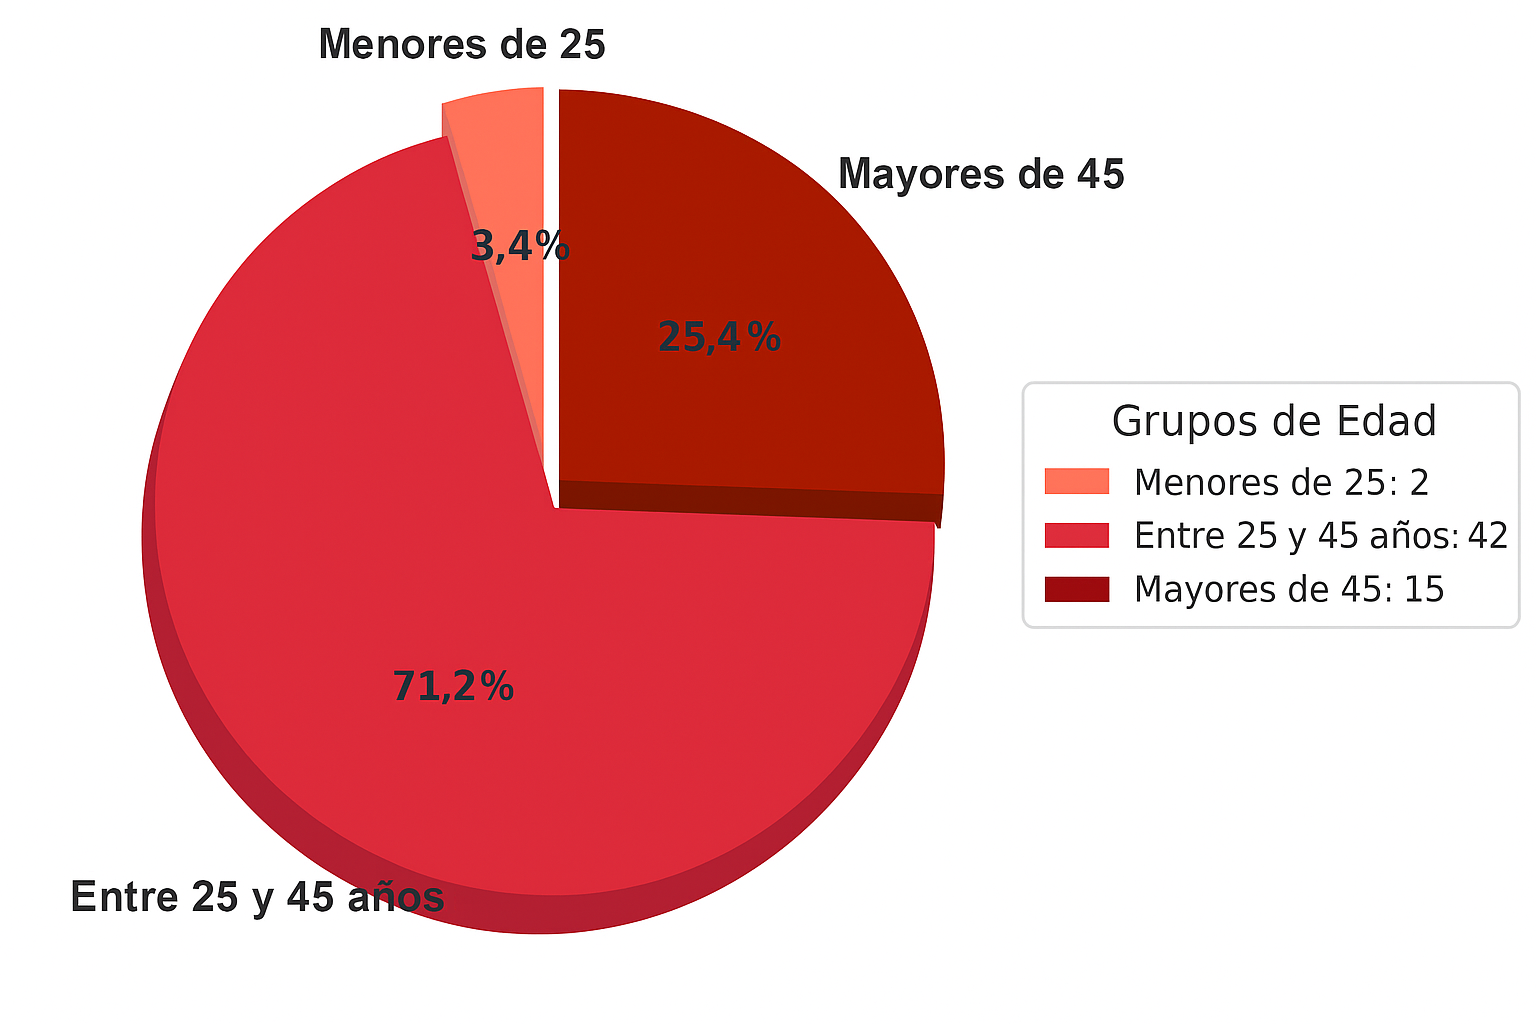
\includegraphics[width=\linewidth]{Fig2.png}
    \caption{Edad del profesorado participante.}
    \label{fig2}
    \source{Elaboración propia.}
    \end{minipage}
\end{figure}

Es importante reseñar que, dadas las características de acceso a la profesión, el profesorado extremeño menor de 25 años representa una porción menos significativa del total del profesorado en activo. En cambio, este primer dato es posible compararlo con los años de experiencia, identificando esta vez sí, una mayor predisposición del profesorado con menor experiencia docente. El profesorado de 1 a 5 años representaba el 57.63~\% del total, 34 de los 59 participantes. Destacando en base a las implicaciones tradicionales del videojuego en la sociedad, el número de mujeres participantes, 36, frente al de hombres 23.

En lo respectivo a la situación administrativa, el análisis de las medias y los datos recogidos muestran que la mayoría de inscritos e inscritas, 33 participantes, eran interinos frente a 26 participantes que se encontraban en otras situaciones como comisiones de servicios, funcionarios en prácticas, personal definitivo o contratados.

En relación con el cuerpo docente al que pertenecían, 19 eran maestros y maestras, mientras que el resto era Profesorado de Educación Secundaria 35 y Formación Profesional, 5.

En este sentido, es importante reseñar dos aspectos, el primero de ellos es la relación entre las necesidades detectadas por los Centros de Profesores y Recursos y el interés real del profesorado que, se evidencia en la inscripción y la participación real del profesorado. Mientras que, en segundo lugar, es posible detectar una mayor aceptación entre el profesorado más joven que ha participado en experiencias e investigaciones vinculadas al videojuego durante su formación, y que además se han formado como docentes en un contexto más influenciado por las tecnologías digitales.

\subsection{P2. ¿Qué expectativas tiene el profesorado extremeño en relación con la incorporación de los videojuegos a su formación y práctica educativa?}\label{sec-resumo}
Al finalizar cada curso, el profesorado participante pudo evaluar el grado de adecuación del curso en torno a las expectativas previas de formación y la utilidad real de la misma. En concreto en este apartado se valoraba con una escala de 1 al 4, donde uno representa el rango más bajo y 4 el más alto, los siguientes aspectos: necesidad de formación, utilidad para el complemento, utilidad como mérito, competencia profesional y mejora de la práctica docente.

La media combinada de todas las participaciones en el curso arroja resultados altos en las expectativas del profesorado respecto a la necesidad como formación (3,25 sobre 4); la utilidad para el complemento (3,25 sobre 4); así como la utilidad como mérito académico (3,23 sobre 4), la competencia profesional (3,23 sobre 4); y la mejora de la práctica docente (3,63 sobre 4). Destaca así, entre todos los aspectos evaluados, la mejora de la práctica docente como la expectativa mejor valorada.

Destaca que, entre todos los aspectos evaluados, las mayores expectativas del profesorado eran vinculadas a la mejora de su propia práctica docente.

Aunque el profesorado valora los videojuegos como un posible recurso de interés, los datos recabados muestran que todavía hace falta formación especializada, que exima a los videojuegos de su visión negativa.

\subsection{P3. ¿Qué grado de satisfacción muestran respecto al curso de Aplicación de los videojuegos en el ámbito educativo?}\label{sec-secoes}
El grado de satisfacción en este tipo de formaciones se estructura en torno a aspectos muy diversos, pues mide aspectos que van desde la duración de las sesiones a los objetivos y contenidos trabajados. Por ese motivo, y para poner en perspectiva toda la intervención, se muestran las respuestas individuales y sus resultados combinados en todos los apartados de este campo (\Cref{tbl2}).

\begin{table}[htbp]
\caption{Grado de satisfacción de los participantes.}
\label{tbl2}
\centering
\begin{tabular}{llllll}
\toprule
Satisfacción/Edición & 1ª Edición & 2ª Edición & 3ª Edición & 4ª Edición & Media General \\ 
 \midrule
Duración & 4.33 & 3.56 & 4.14 & 3.86 & 3.97 \\
Horario & 4.60 & 4.00 & 4.14 & 4.29 & 4.25 \\
Organización & 4.80 & 4.33 & 4.25 & 4.43 & 4.45 \\
Materiales y equipamientos & 4.93 & 4.33 & 4.07 & 4.43 & 4.44 \\
Metodología & 4.67 & 3.89 & 4.07 & 4.71 & 4.33 \\
Ponente & 4.67 & 4.44 & 4.21 & 4.71 & 4.50 \\
Instalaciones & 4.79 & 4.33 & 4.32 & 4.86 & 4.57 \\
Convivencia & 4.80 & 4.38 & 4.46 & 4.86 & 4.62 \\
Diseño del curso & 4.80 & 3.78 & 4.18 & 4.86 & 4.40 \\
Objetivos & 4.73 & 3.78 & 4.11 & 5.00 & 4.40 \\
Contenidos & 4.67 & 3.67 & 4.11 & 5.00 & 4.36  \\
\bottomrule
\end{tabular}
\source{Elaboración propia.}
\end{table}

Aunque posteriormente en los comentarios cualitativos se recibieron algunas sugerencias o valoraciones negativas sobre el apartado metodológico u organizativo, lo cierto es que el análisis de las medias muestra altos grados de satisfacción en todos los ítems evaluados, detectando solo una bajada de la misma en la 2ª edición, la única en la que la media de respuesta bajó de los 4 puntos sobre 5. A colación de los datos obtenidos se puede señalar que el profesorado ha adquirido las habilidades necesarias para la implementación didáctica del videojuego en el aula. No obstante, las puntuaciones indican que deberían mejorarse las distribuciones horarias y la duración de las sesiones para que la formación sea más efectiva.

A nivel general estos resultados muestran una mayor motivación del profesorado frente a la tarea de introducir videojuegos en el aula, que podría traducirse en un mayor porcentaje de aplicación-introducción didáctica.

\subsection{P4.¿Se adecua este tipo de formación a sus puestos de trabajo y a la formación profesional que los docentes perciben como necesaria?}\label{sec-format-simple}
La adecuación de la formación al puesto de trabajo y a la formación profesional de los docentes es uno de los apartados más interesantes de nuestro estudio, pues permite evaluar la percepción del profesorado sobre la relación final entre la formación recibida y la tecnología enunciada con su labor docente. En concreto, en este trabajo se enuncia la percepción del profesorado sobre a la posible utilización de los videojuegos en el aula.

De nuevo, se utiliza la media para evaluar tres aspectos: adecuación al puesto de trabajo, formación personal y formación profesional. (Ver \Cref{tbl3}).

\begin{table}[htbp]
\caption{Adecuación de la formación.}
\label{tbl3}
\centering
\begin{tabular}{llllll}
\toprule
Adecuación & 1ª Edición & 2ª Edición & 3ª Edición & 4ª Edición & Media General \\ 
 \midrule
Puesto trabajo & 4.73 & 3.67 & 3.89 & 5 & 4.32 \\
Formación personal & 4.6 & 3.89 & 3.93 & 5 & 4.36 \\
Formación profesional & 4.67 & 4 & 4.07 & 5 & 4.44 \\
\bottomrule
\end{tabular}
\source{Elaboración propia.}
\end{table}

El profesorado ha interpretado siempre la adecuación de esta formación y de la tecnología utilizada con una valoración alta, que arroja medias en torno al 4,3 y el 4,4 en cada aspecto evaluado, poniendo de relevancia la adecuación de esta formación a los intereses y demandas actuales del profesorado.

\subsection{P5. ¿Qué valoración media recibe la actividad de formación?}\label{sec-links}
La estructura de los CPR está muy interesada en obtener una valoración de cada actividad realizada ya que esto les permite identificar qué cursos son susceptibles de repetirse o trasladarse a otras demarcaciones. En el caso de esta propuesta, la reedición del curso en 4 ediciones es ya un aval de su buena recepción entre los participantes cuya media de valoración se ubica en el 4,46 sobre 5 puntos posibles. Una relación de todas las ediciones se expone en la siguiente figura (Ver \Cref{fig3}).

\begin{figure}
    \centering
    \begin{minipage}{0.6\linewidth}
    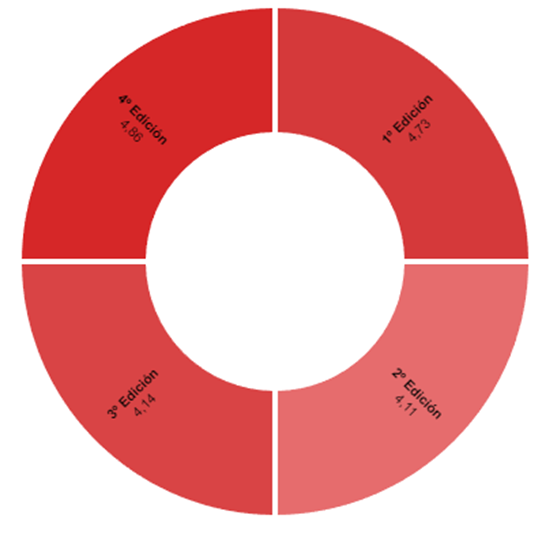
\includegraphics[width=\linewidth]{Fig3.png}
    \caption{Valoración media de la actividad por edición del curso.}
    \label{fig3}
    \source{Elaboración propia.}
    \end{minipage}
\end{figure}

Las puntuaciones muestran que la formación recibe unas valoraciones elevadas, cercanas al máximo. No obstante, tanto la primera, como la segunda edición obtienen puntuaciones menores que las últimas, algo que se vincula a los cambios posteriormente realizados en la misma; percibiéndose una consolidación del modelo formativo.

\subsection{P6. ¿Qué percepciones individuales tiene el profesorado extremeño sobre el desarrollo de este curso? ¿Qué propuestas de mejora o evaluaciones cualitativas realizan?}\label{sec-outras-estr}
Las percepciones individuales del profesorado permiten analizar de forma cualitativa la validez e interés del curso, así como desarrollar mejoras en su implementación y futuras ediciones. En este sentido, la edición con componente virtual recibió algunas críticas negativas respecto a la modalidad de impartición y la duración de esta: “\textit{PCPR1: la organización de las sesiones ha resultado bastante improductiva. Muchos tiempos conectados solo mirando una cámara cuando podrían haberse organizado como actividades fuera de conexión...”, la mayoría de ellas, felicitando el trabajo realizado, pero reseñando la necesidad de una mayor carga horaria y la conveniencia de una modalidad presencial: “PCPR4: · la duración del curso debería ser mayor, el ámbito de los videojuegos da mucho de sí. Sería muy recomendable alguna sesión presencial”. O “PCPR10: combinar sesiones presenciales y online (sabemos que por esta situación ha tenido que ser así). Hemos tenido una visión general de todo lo que podemos llegar hacer y de muchos videojuegos que hay y que podemos introducir en el aula. Sería positivo aumentar el número de horas del curso, centrarnos en determinados videojuegos o recursos para gamificar el aula y llevarlos a la práctica. Mi enhorabuena a todos los ponentes del curso por su planteamiento ha sido un curso muy interesante, dinámico, han conseguido motivarnos y estar ahí pendiente todas las semanas. Se lo han preparado muy bien y nos han ofrecido muchos recursos. Gracias.”}

Del mismo modo, el planteamiento también fue reconsiderado, al responder los participantes que era necesario disponer de conocimientos previos para poder llevar a cabos sus propias experiencias de aula: \textit{“PCPR20: el curso ha estado muy bien y he aprendido muchas cosas, pero no estaba enfocado como había esperado, “PCPR23: se ha tratado poco la aplicación de videojuegos en las aulas...” “PCPR32: considero que el curso va destinado a profesores que ya tienen cierta experiencia y conocimiento de los videojuegos a nivel personal, para los que no la tenemos, es difícil de aprovechar” PCPR33: “las primeras clases las centraría mucho más en la gente que no conoce el tema”}.

Teniendo en cuenta la gran cantidad de participantes que consideraba más adecuado desarrollar sesiones presenciales y con la mejora de la situación sociosanitaria, los siguientes cursos se desarrollaron en modalidades con componente presencial, lo que mejoró susceptiblemente las valoraciones recibidas, eliminando las quejas por la modalidad online:

Del mismo modo, la formación presencial se reenfocó, dejando menos espacio a la improvisación y a los conocimientos previos del profesorado y dirigiéndose a una herramienta específica como RPG Maker, sobre la que se desarrollaban las propuestas de videojuegos dentro de las propias sesiones, con apoyo de ponentes y organizadores, lo que arrojó un mayor grado de satisfacción y aceptación entre los participantes, que ahora solo deseaban más tiempo \textit{“PCPR48: mayor duración para aumentar el tiempo de práctica” y satisfacción “PCPR38: el curso ha estado muy bien y he aprendido muchas cosas...”, PCPR39: bien organizado y perfecto en su desarrollo”}.


\subsection{P7. ¿Qué aspectos o elementos del curso fue necesario mejorar o cambiar? ¿Qué elementos identifica cómo determinantes en el proceso de aprendizaje-utilización el profesorado participante?}\label{sec-listas}
Las propuestas y valoraciones del profesorado participante provocaron la modificación paulatina del contenido del curso, entre los aspectos o elementos determinantes a la hora de mejorar y adaptar esta formación. El profesorado participante siempre encontró la presencialidad como uno de los aspectos más relevantes, motivo por el cual se reestructuró la formación pasando de una formación abierta basada en la utilización de videojuegos comerciales, creadores de videojuegos u otros recursos de forma indistinta, a una formación cerrada, centrada en el diseño de videojuegos con un software específico, fundamentada en el apoyo docente, resultando ser la metodología con la que más cómodo se encontraba el profesorado.

En cuanto al componente de presencialidad, el curso se ofertó en primer lugar con una modalidad online (Ver \Cref{fig4}).

\begin{figure}
    \centering
    \begin{minipage}{0.75\linewidth}
    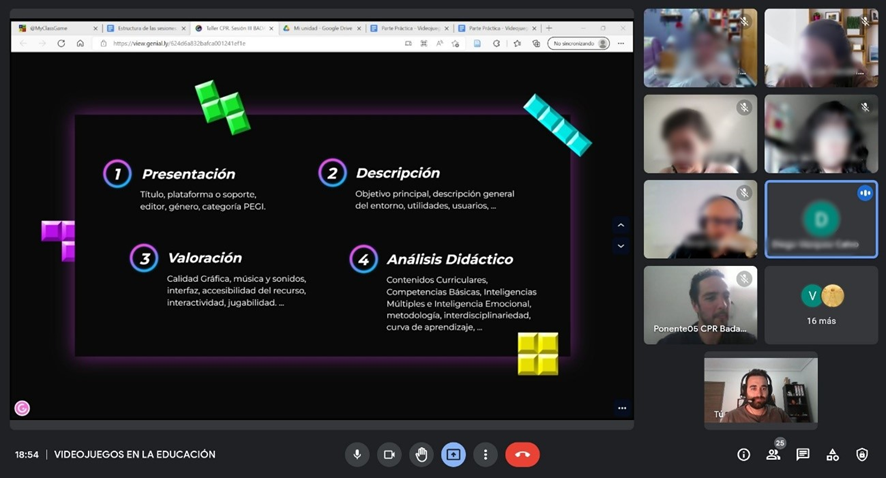
\includegraphics[width=\linewidth]{Fig4.png}
    \caption{Ejemplo de una sesión virtual del curso.}
    \label{fig4}
    \source{Captura de pantalla de la presentación y la sala de videoconferencia, elaboración propia.}
    \end{minipage}
\end{figure}

Posteriormente se descartó esta modalidad en beneficio de una híbrida que, aunque respondió a las demandas del profesorado de mayor presencialidad, resultó confusa y menos práctica de lo esperado, motivo por el cual se decidió pasar a una modalidad completamente presencial. Este hecho, ligado a las demandas del profesorado de más tiempo, así como al éxito y la encadenación de sucesivas ediciones dentro de los planes de formación de los CPR, permite afirmar que el interés por los videojuegos del profesorado es alto y está condicionado al tipo de formación y los ajustes realizados en la misma.

Determinante resulta también ofrecer a los docentes la posibilidad de crear su propio juego desde cero, adaptando este a sus contenidos, ideas o intenciones, algo que no se realizaba en la primera edición en la que el abanico de posibilidades era más amplio, eligiendo juegos comerciales, buscando juegos personalizados a cada profesor, etcétera. La experiencia y las valoraciones del profesorado han demostrado que la mejor opción fue la de dotarles de una herramienta completa con la que crear desde cero estos recursos.

Por último, la adquisición de conocimientos previos, el propio hecho de haber jugado a videojuegos o asistir a una formación como esta, permite al profesorado conocer mejor los videojuegos, familiarizándose con sus mecánicas y sistemas, para poder reproducir estos con mayor éxito. En este sentido, es significativo el hecho de que, para desarrollar otras metodologías actuales como la gamificación, es necesario conocer los diferentes elementos y componentes de juego que luego se extraerán o utilizarán en las clases. Del mismo modo, empatizar con el alumnado, conocer su intereses y aficiones permite al profesorado alcanzar sus objetivos con mayor probabilidad de éxito.

\section{Discusiones y conclusiones}\label{sec-figuras-tabelas}
Esta investigación permite enunciar una serie de evidencias en torno a la formación del profesorado en la utilización de videojuegos como recurso educativo, así como contrastar la necesidad de formación específica expuesta previamente por otras investigaciones \cite{marin2022videojuegos,gonzalez2023diseno}, reforzando la idea de la necesidad de formación y la validez de un modelo como el expuesto que se fundamenta en dotar al profesorado de herramientas para crear sus propios videojuegos \cite{gonzalez2023diseno}.

Del mismo modo, se hace posible contrastar el perfil del profesorado que se interesa por los videojuegos y las metodologías didácticas de implementación y aplicación en el aula, compuesto mayoritariamente de profesores jóvenes o que se encuentran en sus primeros años de experiencia docente \cite{gerardo2022videojuego}.

La buena aceptación y la continuidad de esta propuesta de formación dentro de los planes de formación del profesorado de la comunidad autónoma de Extremadura enuncia la validez y actualidad de los videojuegos como medios de enseñanza dentro de las aulas extremeñas, así como el interés del profesorado, siendo este un punto de partida esperanzador para esta y otras investigaciones, ya que evidencia la buena acogida que tendrá en las aulas la implementación del videojuego, sentando las bases para dotar al profesorado de las herramientas y recursos para utilizarlos.

El hecho de que este modelo de formación se fundamente en el Plan Marco de Formación Permanente del Profesorado de la Comunidad Autónoma de Extremadura \cite{extremadura2022plan}, constituye en sí una garantía de la validez y actualidad de las formaciones realizadas que se fundamenta en la responsabilidad de las administraciones que establece la Ley Orgánica 3/2020 de 29 de diciembre, LOMCE, para desarrollar la formación continua del profesorado, en base a la adecuación de los conocimientos y la evolución de las ciencias y las didácticas \cite{ministerio2020ley}.

La reedición de hasta 4 ediciones del curso de formación en los Aspectos didácticos del videojuego, formación e implementación, ha servido no solo para formar al profesorado, sino para conocer el interés real de los docentes por programar y crear sus propias experiencias de juego. La evaluación de las distintas formaciones muestra una alta satisfacción del profesorado participante, que no solo manifiesta ver cumplidas sus expectativas, sino que considera la formación satisfactoria y adecuada a su puesto de trabajo. Esto permite que la valoración media de la actividad sea alta y que los autores, en base a las percepciones del profesorado hayan podido identificar y enunciar un modelo de formación específico, detectando: (1) la necesidad de formación específica, (2) desconexión y falta de comprensión respecto al medio de lenguaje y el videojuego como herramienta de comunicación y (3) la mejor predisposición del profesorado a que estos cursos sean presenciales y (4) les permitan crear de ceros sus propios juegos, así como (5) adaptar las formaciones desde la perspectiva del docente y la investigación; y, (6) dotarles de las herramientas, recursos y conocimientos que ellos demandan y necesitan.

Con todo esto, se defiende haber alcanzado un diseño formativo de alto impacto y calidad formativa que tendrá consecuencias en la comunidad educativa y en concreto en el personal docente de la comunidad autónoma de Extremadura, su alumnado y el desarrollo de futuras experiencias o investigaciones dentro y fuera de nuestro espacio educativo.

\subsection{Limitaciones}\label{sec-quotesandfootnotes}
Respecto a las limitaciones del estudio se identifica el tamaño de la muestra como uno de los aspectos más limitantes; no obstante, conviene destacar que los datos recogidos, al tratarse de profesorado, y por lo tanto especialistas educativos, dotan de mayor valor a la investigación realizada, permitiendo observar con mayor profundidad y contraste un proceso de formación de interés para la investigación e innovación educativa. Futuras líneas de investigación deben centrarse en el proceso posterior de integración del videojuego que estos docentes realizarán en su práctica docente tras las formaciones, así como en la extrapolación de este modelo formativo a otros contextos educativos regionales e internacionales, fortaleciendo su aplicabilidad y alcance.


\section{Agradecimientos}\label{sec-equacao}
Este trabajo cuenta con el apoyo de la Consejería de Educación, Ciencia y Formación Profesional de la Junta de Extremadura. Entidad de la que son dependientes los Centros de Formación del Profesorado en los que se aprobaron los planes de formación evaluados y a los que pertenece el profesorado participante. En este sentido se declara además que el custodio y recogida de los datos les pertenece y que son estas entidades, quién a través de acuerdo suscrito con los autores, los ceden para esta investigación.

El trabajo, forma parte además de una Tesis Doctoral desarrollada en la Universidad de Extremadura, dentro del Programa de Doctorado (R010) Innovación en Formación del Profesorado. Asesoramiento, Análisis de la Práctica Educativa y TIC en Educación.


\section{Declaración ética}\label{sec-codigos}
Esto documento cuenta con la autorización expresa de los Centros de Profesores y Recursos dependientes de la Consejería de Educación de la Comunidad Autónoma de Extremadura. La recogida de los datos se realiza a través de estos centros, garantizándose la salvaguarda de los datos personales que se entregan anonimizados, expresados a través de las medias de las respuestas voluntarias de los y las participantes en las formaciones impartidas por los propios investigadores, dentro de los planes de formación de cada uno de los centros. El protocolo de recogida de datos sigue las instrucciones del Comité de Bioética de la Universidad de Extremadura y la Declaración de Helsinki.


\printbibliography\label{sec-bib}
% if the text is not in Portuguese, it might be necessary to use the code below instead to print the correct ABNT abbreviations [s.n.], [s.l.]
%\begin{portuguese}
%\printbibliography[title={Bibliography}]
%\end{portuguese}


%full list: conceptualization,datacuration,formalanalysis,funding,investigation,methodology,projadm,resources,software,supervision,validation,visualization,writing,review
\begin{contributors}[sec-contributors]
\authorcontribution{Mario Cerezo-Pizarro}[conceptualization,datacuration,formalanalysis,investigation,methodology,writing,review]
\authorcontribution{Francisco Ignacio Revuelta-Domínguez}[conceptualization,methodology,supervision,review]
\authorcontribution{Jorge Guerra-Antequera}[conceptualization,methodology,investigation,supervision,review]
\end{contributors}

\end{document}

